\subsection{Méthode de la dichotomie}\label{exo:1}

\begin{td-exo}\,
    \begin{enumerate}
        \item Quelle équation souhaite-t-on résoudre pour notre problème d'optimisation?
        Quelles conditions doit-on vérifier sur \(f\) pour appliquer la méthode de la dichotomie?
    
        \item Ecrire l'algorithme de dichotomie et l'appliquer pour trouver le minimum de la fonction
        \(f = x^2 - 2\sin(x)\) sur \(\ff{0,2}\) avec une précision de \(10^{-5}\).
        Comment obtient-on le nombre d'itérations à partir de la précision?
    
        \item Comparer votre code avec l'implémentation de la fonction \texttt{scipy.optimize.bisect}.
    \end{enumerate}
\end{td-exo}

\iftoggle{showsolutions}{
    \begin{td-sol}\,
        \begin{enumerate}
            \item On souhaite résoudre l'équation \(f'(x) = 0\) pour trouver le minimum de \(f\).
            Pour appliquer la méthode de la dichotomie, il faut que \(f\) soit continue et unimodale sur \(\ff{a,b}\).

            On va alors chercher à résoudre \(f'(x) = 0\) pour trouver les points critiques de \(f\).

            \item On commence par importer les librairies nécessaires et définir la fonction \(f\):
            \begin{center}
                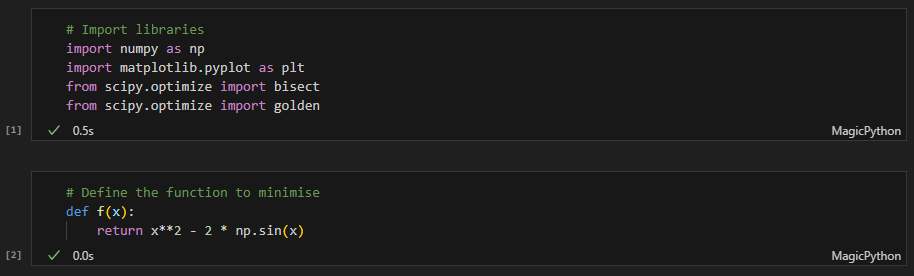
\includegraphics[width=0.8\textwidth]{../assets/code_01_libs_f.png}
            \end{center}
            
            Ensuite on définit la fonction \texttt{dichotomie} qui prend en argument la fonction \(f\), les bornes de l'intervalle \(\ff{a,b}\)
            sur lequel on cherche le minimum et la précision \(\varepsilon\). On l'applique ensuite à notre fonction \(f\):
            \begin{center}
                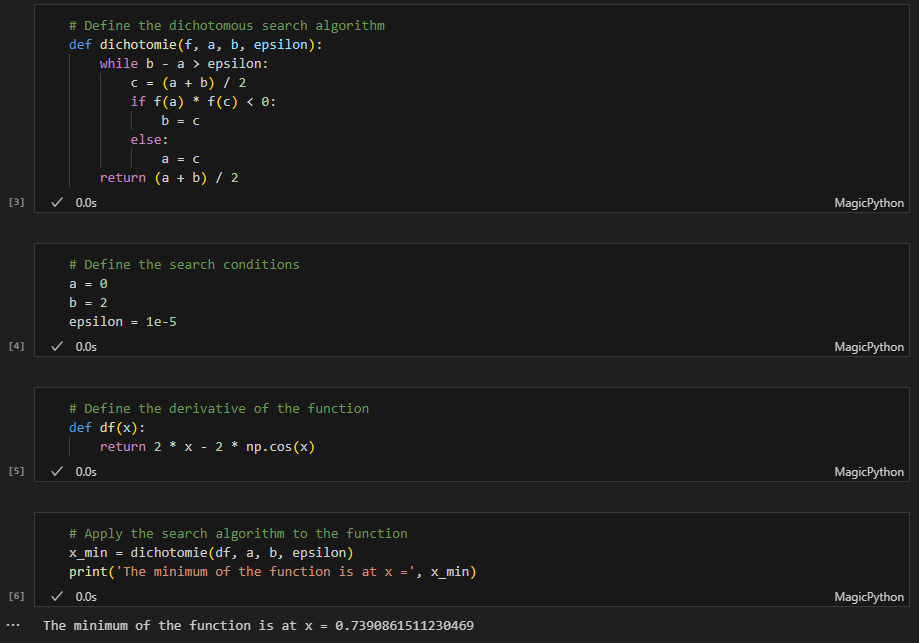
\includegraphics[width=0.8\textwidth]{../assets/code_02_dichotomie.png}
            \end{center}

            Pour obtenir le nombre d'itérations à partir de la précision, on utilise la formule
            \begin{equation*}
                n = \frac{\log(\frac{b - a}{\varepsilon})}{\log(2)},
            \end{equation*}
            où \(n\) est le nombre d'itérations, \(a\) et \(b\) sont les bornes de l'intervalle et \(\varepsilon\) est la précision.
            
            \item On remarque que la méthode de dichotomie de \texttt{scipy.optimize.bisect} donne le même résultat. Un test plus avancé avec des fonctions plus complexes pourrait montrer des différences en termes de performances.
            \begin{center}
                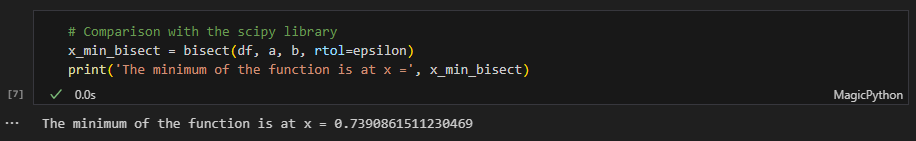
\includegraphics[width=0.8\textwidth]{../assets/code_03_bisect.png}
            \end{center}
        \end{enumerate}
    \end{td-sol}
}{}

\subsection{Méthode de Newton}\label{exo:2}

\begin{td-exo}\,
    \begin{enumerate}
        \item Quelle condition doit vérifier \(f\) pour appliquer la méthode de Newton
        pour le problème d'optimisation? Comment va être formulé l'itéré de Newton dans ce cas?

        \item Ecrire l'algorithme de Newton dans ce cas et l'appliquer à la fonction 
        \(f(x) = x^2 - 2\sin(x)\) avec \(x_0 = 1\).
    \end{enumerate}
\end{td-exo}

\iftoggle{showsolutions}{
    \begin{td-sol}\,
        \begin{enumerate}
            \item Pour appliquer la méthode de Newton, il faut que \(f\) soit de classe \(\mathcal{C}^2\) sur \(\ff{a,b}\).
            L'itéré de Newton est alors donné par
            \begin{equation*}
                x_{k+1} = x_k - \frac{f'(x_k)}{f''(x_k)}.
            \end{equation*}

            \item On définit la fonction \texttt{newton} qui prend en argument la dérivée
            première et seconde de \(f\), la valeur initiale \(x_0\) et la précision \(\varepsilon\).
            On l'applique ensuite à notre fonction \(f\):
            \begin{center}
                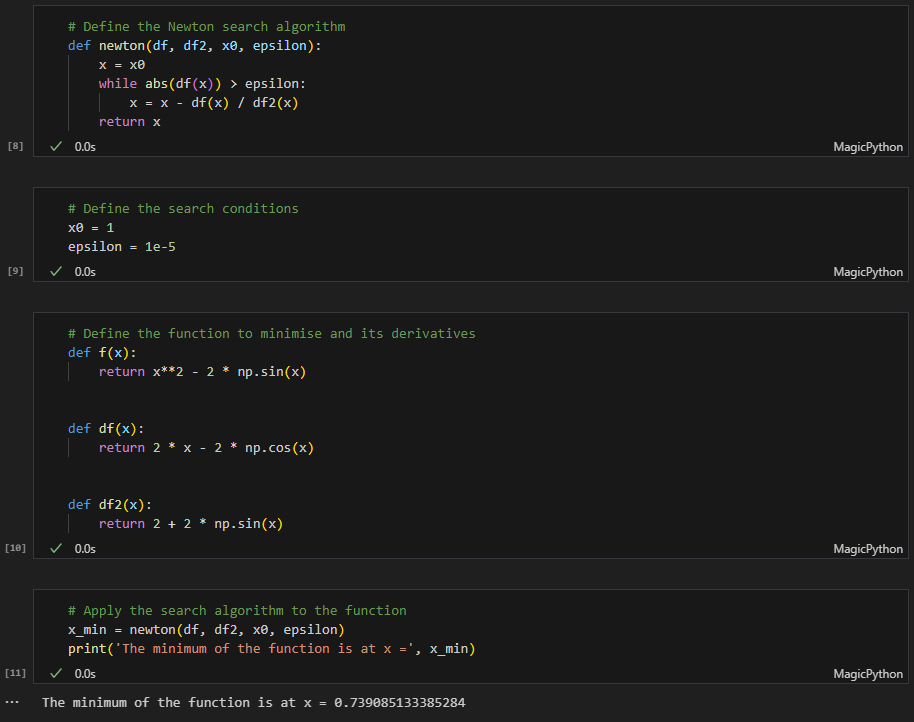
\includegraphics[width=0.8\textwidth]{../assets/code_04_newton.png}
            \end{center}

            On remarque que la méthode de Newton converge plus rapidement que la méthode de dichotomie. 
            Cependant, elle nécessite des conditions plus restrictives sur la fonction \(f\). 
            Dans le cas de la dichotomie, \(f\) doit être unimodale, tandis que pour Newton, 
            \(f\) doit être deux fois dérivable.
        \end{enumerate}
    \end{td-sol}
}{}

\subsection{Méthode de la section dorée}\label{exo:3}

\begin{td-exo}\,
    \begin{enumerate}
        \item Ecrire l'algorithme et l'appliquer à la fonction \(f(x) = x^2 - 2\sin(x)\) sur \(\ff{0,2}\)

        \item Comparer votre code avec l'implémentation de la fonction \texttt{scipy.optimize.golden}.

        \item Comparer les 3 méthodes pour \(f = -\frac1x +\cos(x)\) sur \(\ff{a,b} = \ff{2,4}\)
        ou pour \(x_0 = 2.5\) au niveau du nombre d'itérations et du temps de calcul.

        Représenter le graphique de la fonction en plaçant les résultats des itérations successives
        de Newton.
    \end{enumerate}
\end{td-exo}

\iftoggle{showsolutions}{
    \begin{td-sol}\,
        \begin{enumerate}
            \item On définit la fonction \texttt{golden} qui prend en argument la fonction \(f\), 
            les bornes de l'intervalle \(\ff{a,b}\) sur lequel on cherche le minimum et la
            précision \(\varepsilon\). On l'applique ensuite à notre fonction \(f\):
            \begin{center}
                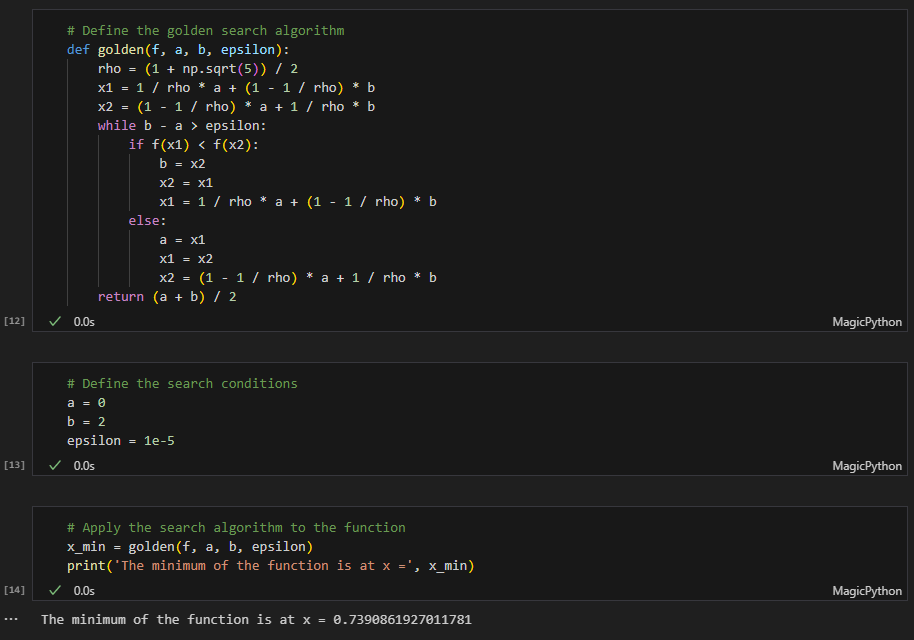
\includegraphics[width=0.8\textwidth]{../assets/code_05_golden.png}
            \end{center}

            \item On remarque que la méthode de la section dorée de \texttt{scipy.optimize.golden} 
            donne le même résultat. Un test plus avancé avec des fonctions plus complexes
            pourrait montrer des différences en termes de performances.
            \begin{center}
                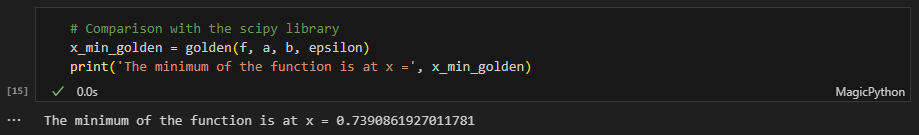
\includegraphics[width=0.8\textwidth]{../assets/code_06_golden.png}
            \end{center}

            \item On définit la fonction \(f = -\frac1x +\cos(x)\) et on applique les 3 méthodes
            pour trouver le minimum sur \(\ff{2,4}\) avec \(x_0 = 2.5\). On compare
            les 3 méthodes en termes de nombre d'itérations et de temps de calcul.

            On représente graphiquement les itérations successives des 3 méthodes.
            \begin{center}
                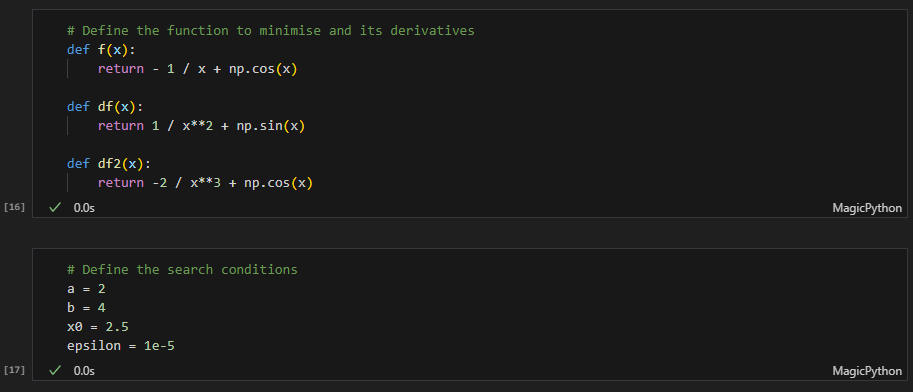
\includegraphics[width=0.8\textwidth]{../assets/code_07_compare.png}
            \end{center}
            
            \begin{center}
                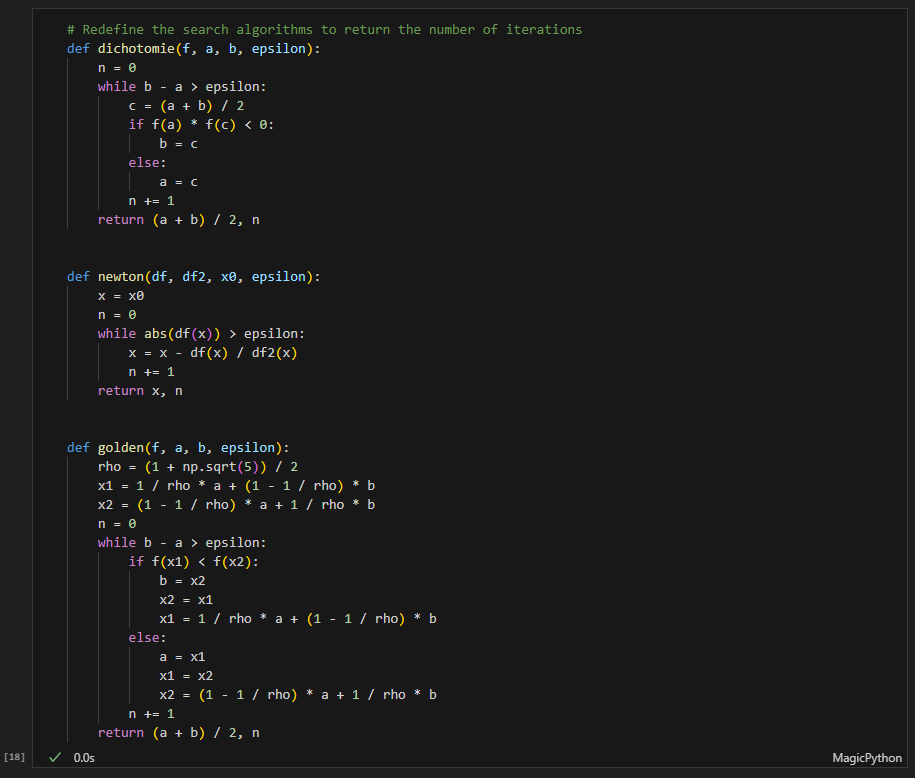
\includegraphics[width=0.8\textwidth]{../assets/code_08_redefine.png}
            \end{center}
            
            \begin{center}
                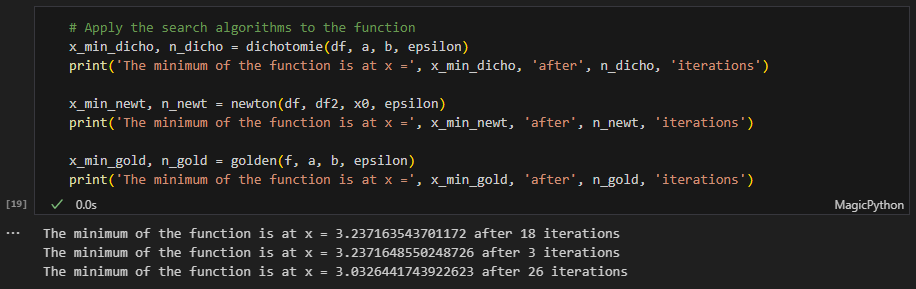
\includegraphics[width=0.8\textwidth]{../assets/code_09_results.png}
            \end{center}
            
            \begin{center}
                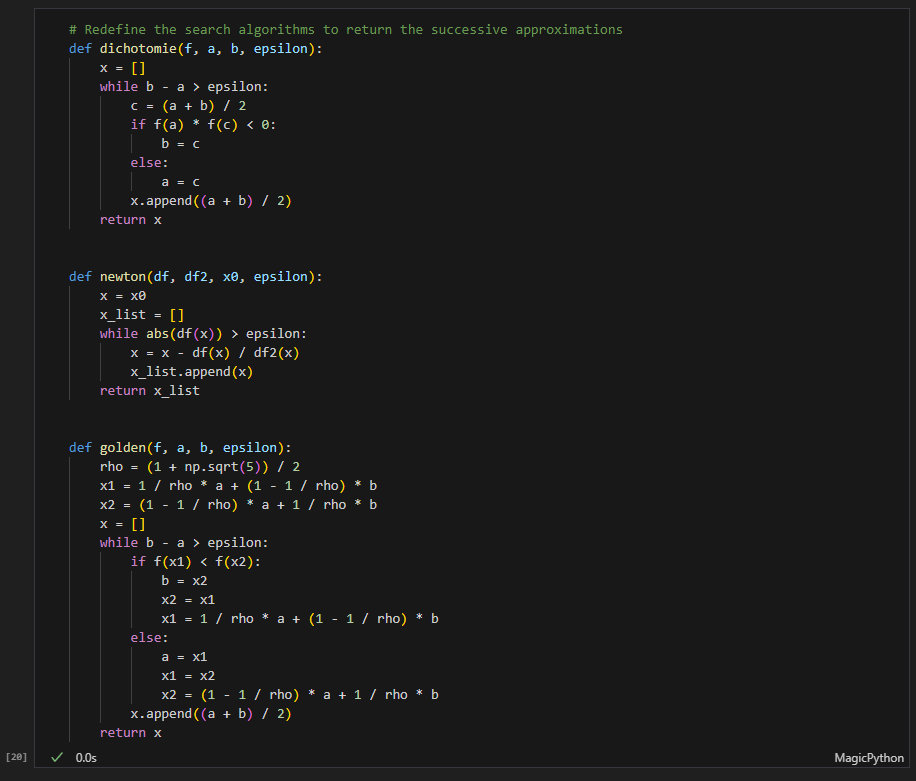
\includegraphics[width=0.8\textwidth]{../assets/code_10_redefine.png}
            \end{center}
            
            \begin{center}
                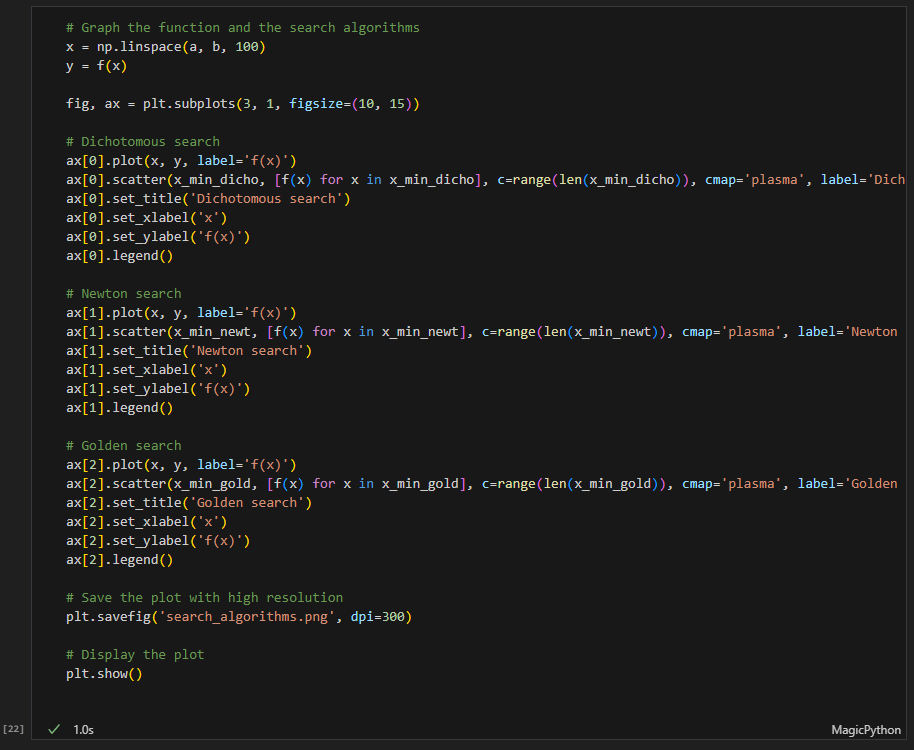
\includegraphics[width=0.8\textwidth]{../assets/code_11_graph.png}
            \end{center}
            
            \begin{center}
                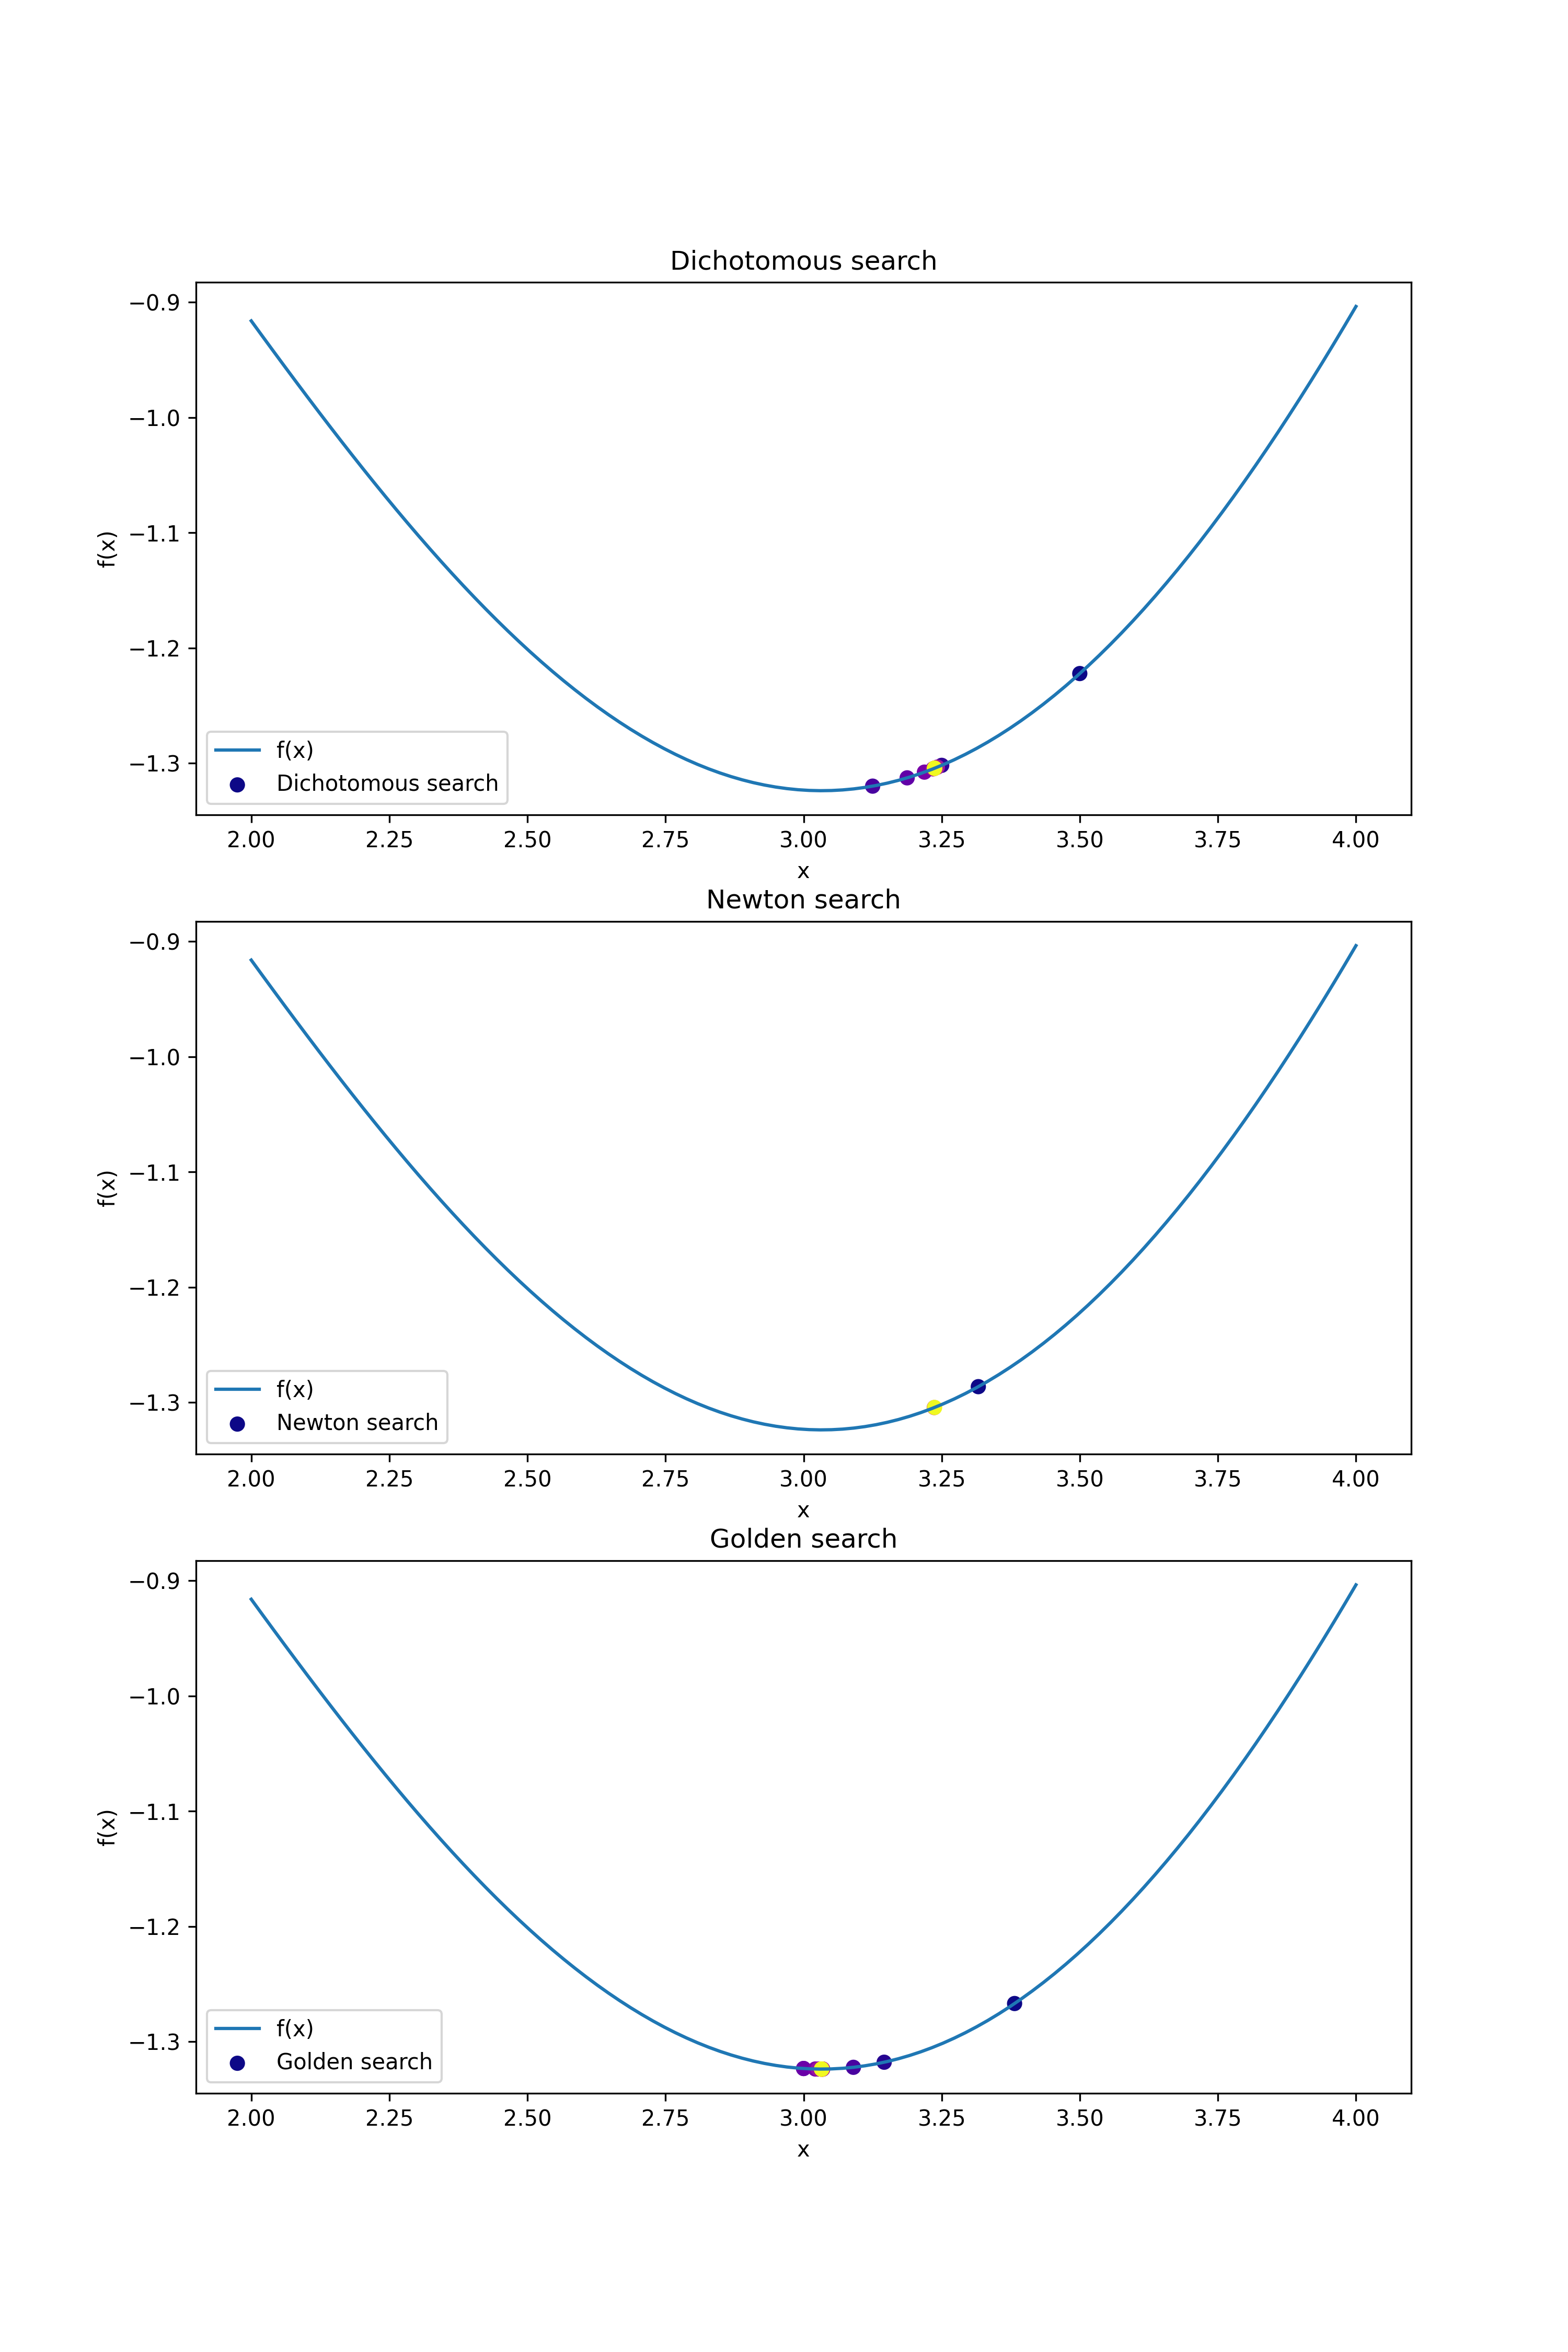
\includegraphics[width=0.8\textwidth]{../assets/code_12_graph.png}
            \end{center}
        \end{enumerate}
    \end{td-sol}
}{}